\selectlanguage{english}%

\chapter{Resultados} \label{capRes}
\epigraph{O destino é inexorável}{Bernard Cornwell}

O modelo fuzzy desenvolvido a partir das seções anteriores foi simulado utilizando o software MATLAB e implementado na bancada real via CLP Rockwell. As seções a seguir apresentam os resultados obtidos em cada caso.

\section{Simulações} \label{secAnalise}
A planta de quatro-tanques, como apresentada no \jhhref{capDescSis}{Capítulo}, compõe um sistema capaz de ilustrar diversas dinâmicas para suas variáveis de processo. Assim, são escolhidas uma configuração em \textbf{fase mínima }e outra em \textbf{fase não-mínima} e a partir delas a modelagem e o controlador fuzzy são desenvolvidos. 

\subsection{Fase Mínima}
Nesta configuração a maior parte do fluído que saí das bombas é direcionado diretamente para os tanques controlados, ou seja $\gamma_i > 0.5$. A \jhhref{tabFaseMinima}{Tabela} a seguir apresenta suas especificações.

\begin{table}[!ht]
	\caption{Parâmetros da planta em fase mínima.}
	\label{tabFaseMinima}
	\small
	\centering
	\scalebox{1}{
		\begin{tabular}{|c|c|}
			\hline
			\multicolumn{2}{|c|}{Especificações Iniciais da Planta} \\
			\hline
			A1, A3 $(cm^2)$ & 28 \\ \hline
			A2, A4 $(cm^2)$ & 32 \\ \hline
			a1, a3 $(cm^2)$ & 0.071 \\ \hline
			a2, a4 $(cm^2)$ & 0.057 \\ \hline
			g $cm/s$ & 981 \\ \hline
			k1 & 3,33 $cm^3/Vs$ \\ \hline
			k2 & 3.35 $cm^3/Vs$ \\ \hline
			$\gamma_1$ & 0.60 \\ \hline
			$\gamma_2$ & 0.70 \\ \hline
			\hline
		\end{tabular}
	}
\end{table}

O \jhhref{eqModNL}{modelo não linear} para esta configuração é:
\begin{equation}
\begin{cases}
\dot{h_{1}} = \frac{1}{28}(0.071\sqrt{1962*h_{3}} + 1,998*v_{1} - a_{1}\sqrt{1962*h_{1}})\\

\dot{h_{2}} = \frac{1}{A_{2}}(a_{4}\sqrt{1962*h_{4}} + \gamma_{2}k_{2}v_{2} - a_{2}\sqrt{1962*h_{2}})\\

\dot{h_{3}} = \frac{1}{A_{3}}((1 - \gamma_{2})k_{2}v_{2} - a_{3}\sqrt{1962*h_{3}})\\

\dot{h_{4}} = \frac{1}{A_{4}}((1 - \gamma_{1})k_{1}v_{1} - a_{4}\sqrt{1962*h_{4}})
\end{cases}
\label{eqFMNL}
\end{equation}

Escolhendo os conjuntos fuzzy \{"baixo","alto"\} e definindo \{5 , 15\} como seus representantes os níveis 1 e 2, por combinação simples obtém-se os seguintes pontos de linearização:
\begin{table}[!ht]
	\caption{Pontos de Operação}
	\small
	\centering
	\scalebox{1}{
		\begin{tabular}{|c|c|c|c|c|c|c|}
			\hline
			Sistema & $\bar{h_1}$ (cm) & $\bar{h_2}$ (cm) & $\bar{h_3}$ (cm) & $\bar{h_4}$ (cm) & $\bar{v_1}$ (v) & $\bar{v_2}$ (v) \\ \hline
			1 & 5 & 5 & 0.0334 & 2.9076 & 3.2321 & 0.5716 \\ \hline
			2 & 5 & 15 & 0.9431 & 1.1033 & 1.9910 & 3.0390 \\ \hline
			3 & 15 & 5 & 0.2229 & 13.0191 & 6.8393 & -1.4773 \\ \hline
			4 & 15 & 15 & 0.1001 & 8.7228 & 5.5982 & 0.9900 \\	\hline
		\end{tabular}
	}
\end{table}

Haverá então quatro regras Se-Então para composição do modelo TS final. As imagens a seguir apresentam a comparação entre os modelos \jhhref{eqModNL}{não-linear}, \jhhref{eqModLinear}{linearizado} em um ponto único e \jhhref{eqTakSugPlanta}{Takagi-Sugeno}:

\begin{figure}[H]
	\centering
	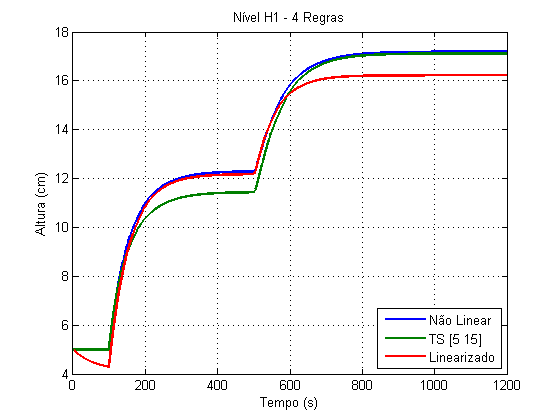
\includegraphics[width=\textwidth]{img/h1_ts2.png}
	\caption{\small Nível do Tanque 1}
	\label{figH1TS2}
\end{figure}

\begin{figure}[H]
	\centering
	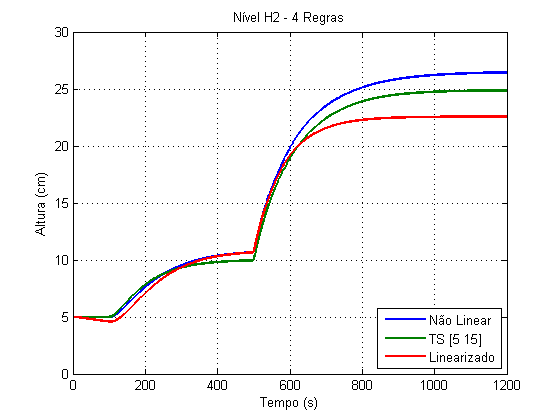
\includegraphics[width=\textwidth ]{img/h2_ts2.png}
	\caption{\small Nível do Tanque 2}
	\label{figH2TS2}
\end{figure}

É notável que o modelo fuzzy representa de modo mais eficiente o sistema. Como dito, o modelo TS pode se aproximar o quanto se desejar do não-linear no qual se baseia. A \jhhref{imgTS5}{Imagem} apresenta um modelo com 5 conjuntos para os dois níveis e a \jhhref{imgTS15}{Imagem} utilizando 15. É importante notar, no entanto, que a complexidade do modelo é exponencial, devido a combinação dos conjuntos das variáveis linguísticas presentes, assim, o primeiro é composto por 25 ($5^2$) regras Se-Então e o segundo por 225 ($15^2$).

\begin{figure}[H]
	\centering
	\begin{tabular}{cc}
		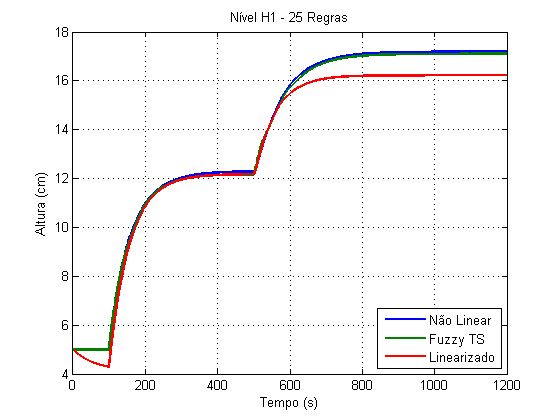
\includegraphics[width=0.5\textwidth,keepaspectratio]{img/h1_ts5.png} &
		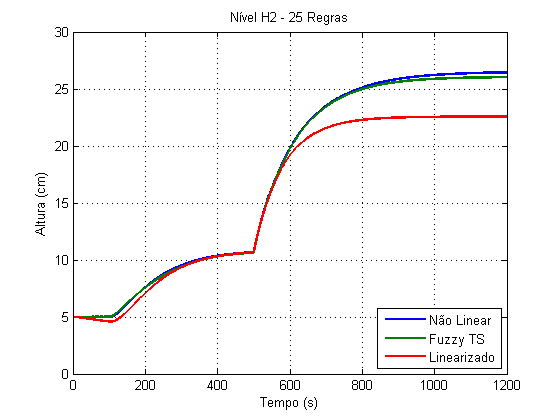
\includegraphics[width=0.5\textwidth,keepaspectratio]{img/h2_ts5.png} \\
		(a) Nível 1 &
		(b) Nível 2
	\end{tabular}
	\caption{\label{imgTS5} Comparação com 25 regras}
\end{figure}

\begin{figure}[H]
	\centering
	\begin{tabular}{cc}
		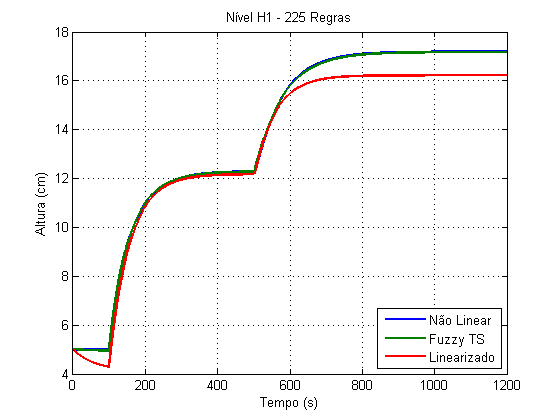
\includegraphics[width=0.5\textwidth,keepaspectratio]{img/h1_ts15.png} &
		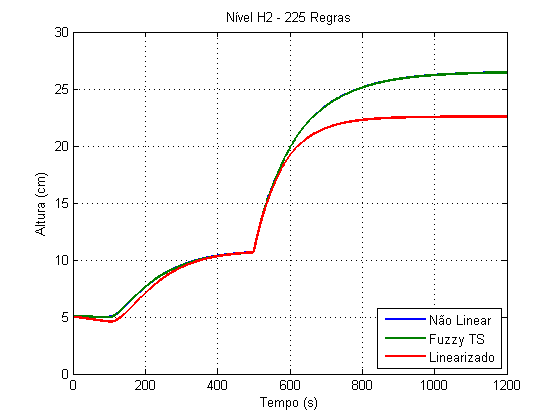
\includegraphics[width=0.5\textwidth,keepaspectratio]{img/h2_ts15.png} \\
		(a) Nível 1 &
		(b) Nível 2
	\end{tabular}
	\caption{\label{imgTS15} Comparação com 225 regras}
\end{figure}

A partir das \jhhref{eqContFuzzy}{Equações} são desenvolvidos os controladores para cada uma das regras. A tabela a seguir apresenta os ganhos obtidos:
\begin{table}[!ht]
	\caption{Ganhos Obtidos}
	\small
	\centering
	\scalebox{1}{
		\begin{tabular}{|c|c|}
			\hline
			Regra & Ganho \\ \hline
			 1 & $ K = 
				\begin{bmatrix}
					-13.1962 & 3.0637 & -3.0992 & 0.1430 & 15.0539 & -1.3580\\
					-5.4607 & -15.2912 & 3.4223 & 0.0239 & 1.6964 & 15.9282
				\end{bmatrix}$ \\[20pt] \hline
			2 & $ K = 
				\begin{bmatrix}
					-12.8885 & 1.0745 & -1.5395 & -0.0323 & 14.9563 & -0.5608\\
					-1.7706 & -13.2431 & 1.0214 & -0.0123 & 0.4755 & 15.4671
				\end{bmatrix}$ \\[20pt] \hline
			3 & $ K = 
				\begin{bmatrix}
					-13.1962 & 3.0637 & -3.0992 & 0.1430 & 15.0539 & -1.3580\\
					-5.4607 & -15.2912 & 3.4223 & 0.0239 & 1.6964 & 15.9282
				\end{bmatrix}$ \\[20pt] \hline
			4 & $ K = 
				\begin{bmatrix}
					-12.8885 & 1.0745 & -1.5395 & -0.0323 & 14.9563 & -0.5608\\
					-1.7706 & -13.2431 & 1.0214 & -0.0123 & 0.4755 & 15.4671
				\end{bmatrix}$ \\[20pt] \hline
		\end{tabular}
	}
\end{table}

Os ganhos são sintonizados para o sistema na forma:
\begin{figure}[H]
	\begin{centering}
		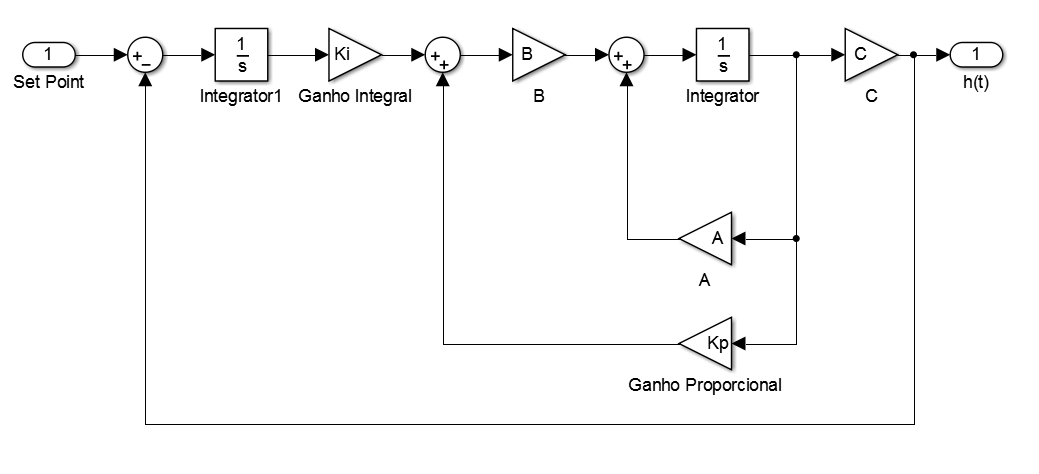
\includegraphics[width=\textwidth]{img/modelo_controlado.png}
		\par\end{centering}
	\caption{\label{figPlantCtrl}Espaço de estados da planta controlada}
\end{figure}

Os níveis controlados podem ser observados nas imagens a seguir:
\begin{figure}[H]
	\centering
	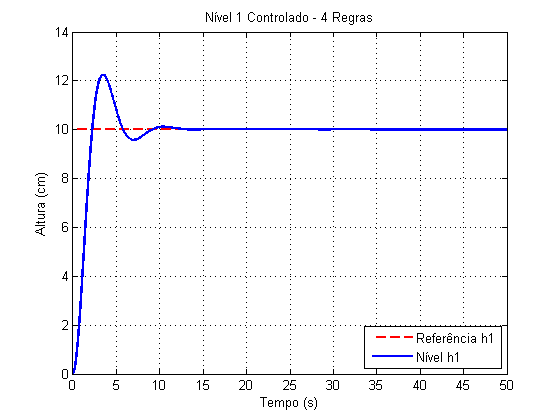
\includegraphics[height=0.35\paperheight ,keepaspectratio]{img/ctrl_h1ts2_free.png}
	\caption{\small Nível H1 Controlado }
	\label{figH1TSCtrl2_free}
\end{figure}

\begin{figure}[H]
	\centering
	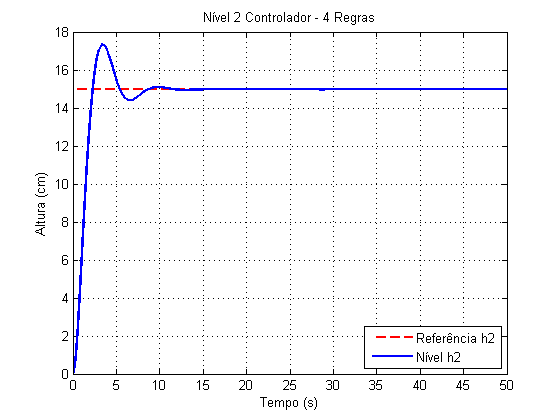
\includegraphics[height=0.35\paperheight ,keepaspectratio]{img/ctrl_h2ts2_free.png}
	\caption{Nível H2 Controlado }
	\label{figH2CtrlTS2_free}
\end{figure}

No entanto, é importante notar que o controle desenvolvido até aqui não leva em consideração os limites(5 V) dos atuadores (bomba). Incluindo-a ao modelo, tem-se:

Para os sistemas das \jhhref{imgTS5}{imagens} e \ref{imgTS15} são sintonizados de forma similar 15 e 225 ganhos e aplicados ao sistema. As imagens a seguir ilustram os resultados obtidos:
\begin{figure}[H]
	\centering
	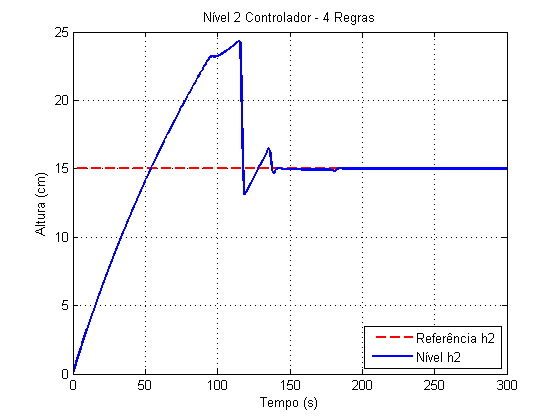
\includegraphics[height=0.35\paperheight ,keepaspectratio]{img/ctrl_h1ts2_ulim.png}
	\caption{\small Nível H1 Controlado - Com saturação do Controlador }
	\label{figH1TSCtrl2_ulim}
\end{figure}

\begin{figure}[H]
	\centering
	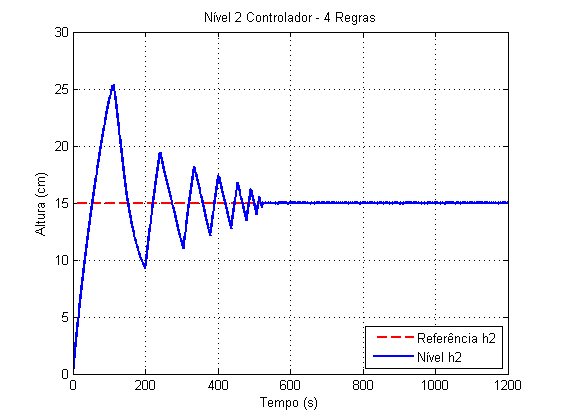
\includegraphics[height=0.35\paperheight ,keepaspectratio]{img/ctrl_h2ts2_ulim.png}
	\caption{Nível H2 Controlado - Com saturação do Controlador }
	\label{figH2CtrlTS2_ulim}
\end{figure}

Para aliviar a ultrapassagem, dada pelo efeito \textit{windup}, utiliza-se a saturação simples dos integradores nos momentos em que as variáveis manipuladas alcançam seus limites de atuação. Os gráficos a seguir ilustram:
\begin{figure}[H]
	\centering
	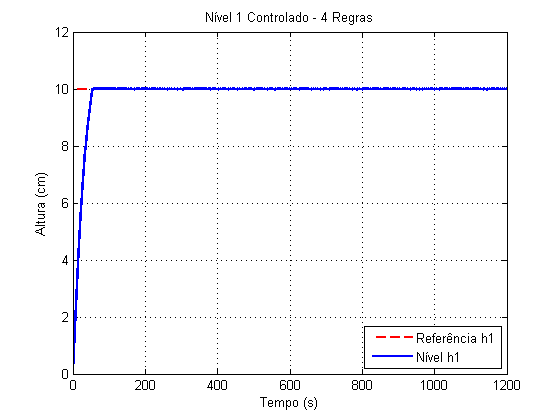
\includegraphics[height=0.35\paperheight ,keepaspectratio]{img/ctrl_h1ts2.png}
	\caption{\small Nível H1 Controlado - Com \textit{Anti-Windup}}
	\label{figH1TSCtrl2}
\end{figure}

\begin{figure}[H]
	\centering
	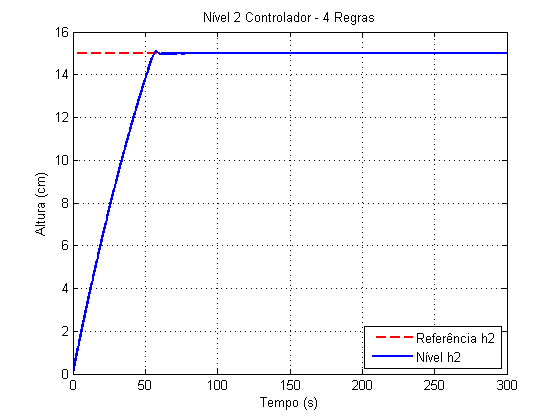
\includegraphics[height=0.35\paperheight ,keepaspectratio]{img/ctrl_h2ts2.png}
	\caption{Nível H2 Controlado - Com \textit{Anti-Windup}}
	\label{figH2CtrlTS2}
\end{figure}

\subsection{Fase Não-Mínima}
Ao contrário da configuração anterior, nesta a maior parte do fluído que saí das bombas é direcionado  para os tanques superiores, ou seja $\gamma_i < 0.5$. A \jhhref{tabFaseNaoMinima}{Tabela} a seguir apresenta as especificações da planta simulada.

\begin{table}[!ht]
	\caption{Parâmetros da planta em fase não-mínima}
	\small
	\centering
	\scalebox{1}{
		\begin{tabular}{|c|c|}
			\hline
			\multicolumn{2}{|c|}{Especificações Iniciais da Planta} \\
			\hline
			A1, A3 $(cm^2)$ & 28 \\ \hline
			A2, A4 $(cm^2)$ & 32 \\ \hline
			a1, a3 $(cm^2)$ & 0.071 \\ \hline
			a2, a4 $(cm^2)$ & 0.057 \\ \hline
			g $cm/s$ & 981 \\ \hline
			k1 & 3,15 $cm^3/Vs$ \\ \hline
			k2 & 3.29 $cm^3/Vs$ \\ \hline
			$\gamma_1$ & 0.43 \\ \hline
			$\gamma_2$ & 0.34 \\ \hline
			\hline
		\end{tabular}
	}
	\label{tabFaseNaoMinima}
\end{table}

O \jhhref{eqModNL}{modelo não linear} para esta configuração é dado por:
\begin{equation}
\begin{cases}
\dot{h_{1}} = \frac{1}{A_{1}}(a_{3}\sqrt{2gh_{3}} + \gamma_{1}k_{1}v_{1} - a_{1}\sqrt{2gh_{1}})\\

\dot{h_{2}} = \frac{1}{A_{2}}(a_{4}\sqrt{2gh_{4}} + \gamma_{2}k_{2}v_{2} - a_{2}\sqrt{2gh_{2}})\\

\dot{h_{3}} = \frac{1}{A_{3}}((1 - \gamma_{2})k_{2}v_{2} - a_{3}\sqrt{2gh_{3}})\\

\dot{h_{4}} = \frac{1}{A_{4}}((1 - \gamma_{1})k_{1}v_{1} - a_{4}\sqrt{2gh_{4}})
\end{cases}
\label{eqFNMNL}
\end{equation}

De forma similar, escolhendo os conjuntos fuzzy \{"baixo","alto"\} e definindo \{5 , 15\} como seus representantes os níveis 1 e 2, tem-se os seguintes pontos de linearização:
\begin{table}[!ht]
	\caption{Pontos de operação}
	\small
	\centering
	\scalebox{1}{
		\begin{tabular}{|c|c|c|c|c|c|c|}
			\hline
			Sistema & $\bar{h_1}$ (cm) & $\bar{h_2}$ (cm) & $\bar{h_3}$ (cm) & $\bar{h_4}$ (cm) & $\bar{v_1}$ (v) & $\bar{v_2}$ (v) \\ \hline
			1 & 5 & 5 & 2.0804 & 1.7175 & 1.8428 & 2.0890 \\ \hline
			2 & 5 & 15 & 0.0321 & 15.9038 & 5.6078 & -0.2595 \\ \hline
			3 & 15 & 5 & 16.9727 & 0.1661 & -0.5730 & 5.9668 \\ \hline
			4 & 15 & 15 & 6.2413 & 5.1525 & 3.1919 & 3.6183 \\	\hline
		\end{tabular}
	}
\end{table}

As imagens a seguir apresenta a comparação entre os modelos \jhhref{eqModNL}{não-linear}, \jhhref{eqModLinear}{linearizado} em um ponto único e \jhhref{eqTakSugPlanta}{Takagi-Sugeno}:

\begin{figure}[H]
	\centering
	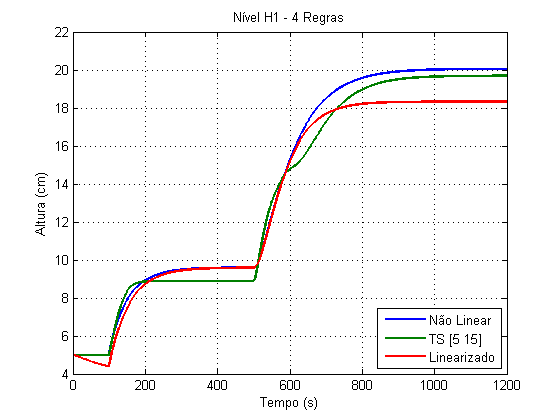
\includegraphics[width=\textwidth]{img/h1_ts2_nm.png}
	\caption{\small Nível do Tanque 1}
	\label{figH1TS2_nm}
\end{figure}

\begin{figure}[H]
	\centering
	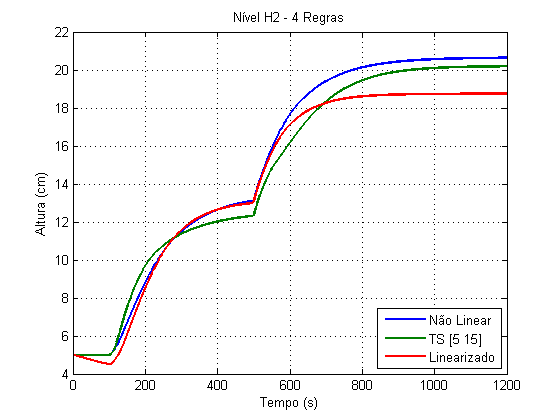
\includegraphics[width=\textwidth]{img/h2_ts2_nm.png}
	\caption{\small Nível do Tanque 2}
	\label{figH2TS2_nm}
\end{figure}

Percebe-se novamente que o sistema Takagi-Sugeno apresenta resultados mais próximos do real na maior parte do tempo. Aumentando a quantidade de regras obtém-se resultados cada vez melhores. As imagens a seguir apresentam os modelos com 5 e com 15 pontos linearização

\begin{figure}[H]
	\centering
	\begin{tabular}{cc}
		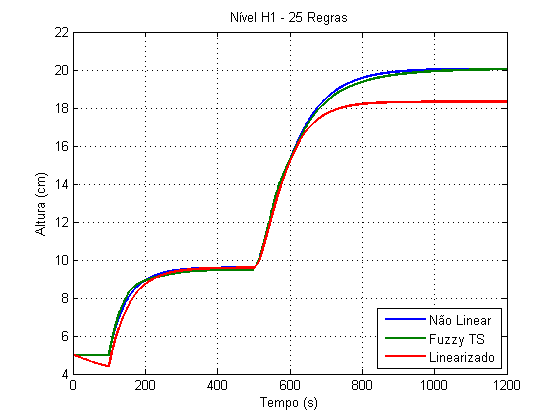
\includegraphics[width=0.5\textwidth,keepaspectratio]{img/h1_ts5_nm.png} &
		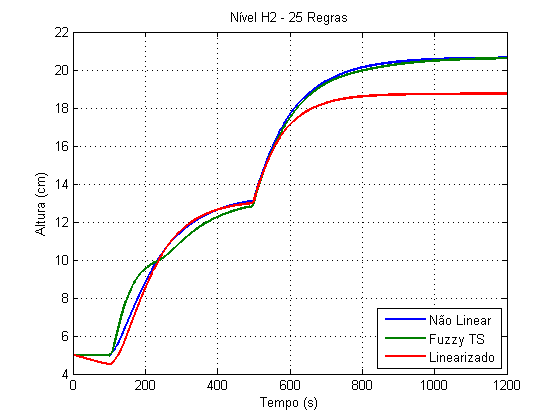
\includegraphics[width=0.5\textwidth,keepaspectratio]{img/h2_ts5_nm.png} \\
		(a) Nível 1 &
		(b) Nível 2
	\end{tabular}
	\caption{\label{imgTS5_nm} Comparação com 25 regras TS}
\end{figure}

\begin{figure}[H]
	\centering
	\begin{tabular}{cc}
		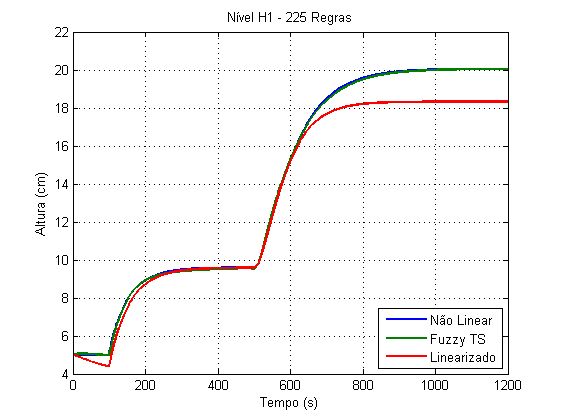
\includegraphics[width=0.5\textwidth,keepaspectratio]{img/h1_ts15_nm.png} &
		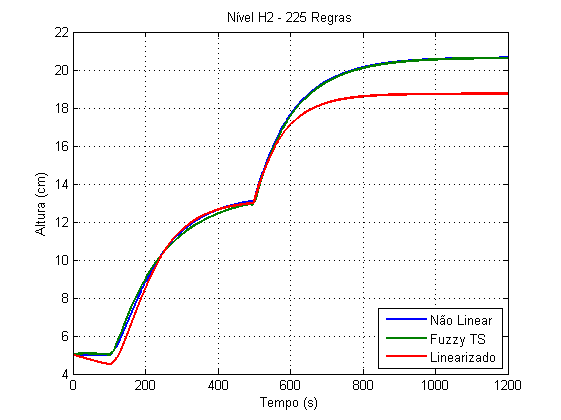
\includegraphics[width=0.5\textwidth,keepaspectratio]{img/h2_ts15_nm.png} \\
		(a) Nível 1 &
		(b) Nível 2
	\end{tabular}
	\caption{\label{imgTS15_nm} Comparação com 225 regras TS}
\end{figure}

A partir das \jhhref{eqContFuzzy}{Equações} são desenvolvidos os controladores para cada uma das regras. A tabela a seguir apresenta os ganhos obtidos:
\begin{table}[!ht]
	\caption{Ganhos Obtidos}
	\small
	\centering
	\scalebox{1}{
		\begin{tabular}{|c|c|}
			\hline
			Regra & Ganho \\ \hline
			1 & $ K = 
			\begin{bmatrix}
			490.5249 & -805.4358 & 366.4860 & -439.5865 & 0.3923 &  19.9419 \\
			-385.9505 & 484.5975 & -230.7682 & 333.2462 & 10.4116 & -4.9420
			\end{bmatrix}$ \\[20pt] \hline
			2 & $ K = 
			\begin{bmatrix}
			0.9652 & -1.5850 & 0.7224 & -0.8567 & -0.0047 & 0.0357 \\
			-0.2384 & 0.3018 & -0.1458 & 0.2055 & 0.0069 &  -0.0025
			\end{bmatrix}$ \\[20pt] \hline
			3 & $ K = 
			\begin{bmatrix}
			490.5249 & -805.4358 & 366.4860 & -439.5865 & 0.3923 &  19.9419 \\
			-385.9505 & 484.5975 & -230.7682 & 333.2462 & 10.4116 & -4.9420
			\end{bmatrix}$ \\[20pt] \hline
			4 & $ K = 
			\begin{bmatrix}
			 0.9652 & -1.5850 & 0.7224 & -0.8567 & -0.0047 & 0.0357 \\
			-0.2384 & 0.3018 & -0.1458 & 0.2055 & 0.0069 & -0.0025
			\end{bmatrix}$ \\[20pt] \hline
		\end{tabular}
	}
\end{table}

Os níveis controlados podem ser observados nas imagens a seguir:
\begin{figure}[H]
	\centering
	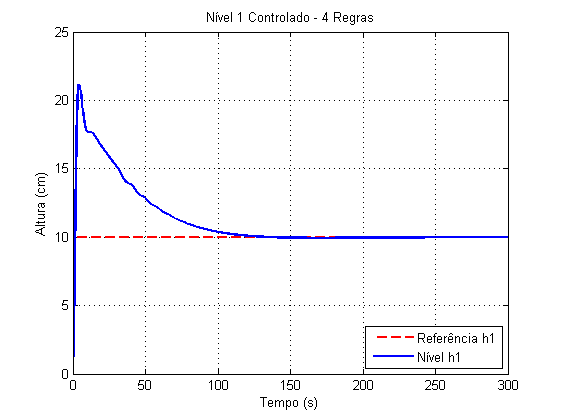
\includegraphics[width=\textwidth]{img/nm_ctrl_h1ts2_free.png}
	\caption{\small Nível H1 Controlado }
	\label{figH1TSCtrl2_free_nm}
\end{figure}

\begin{figure}[H]
	\centering
	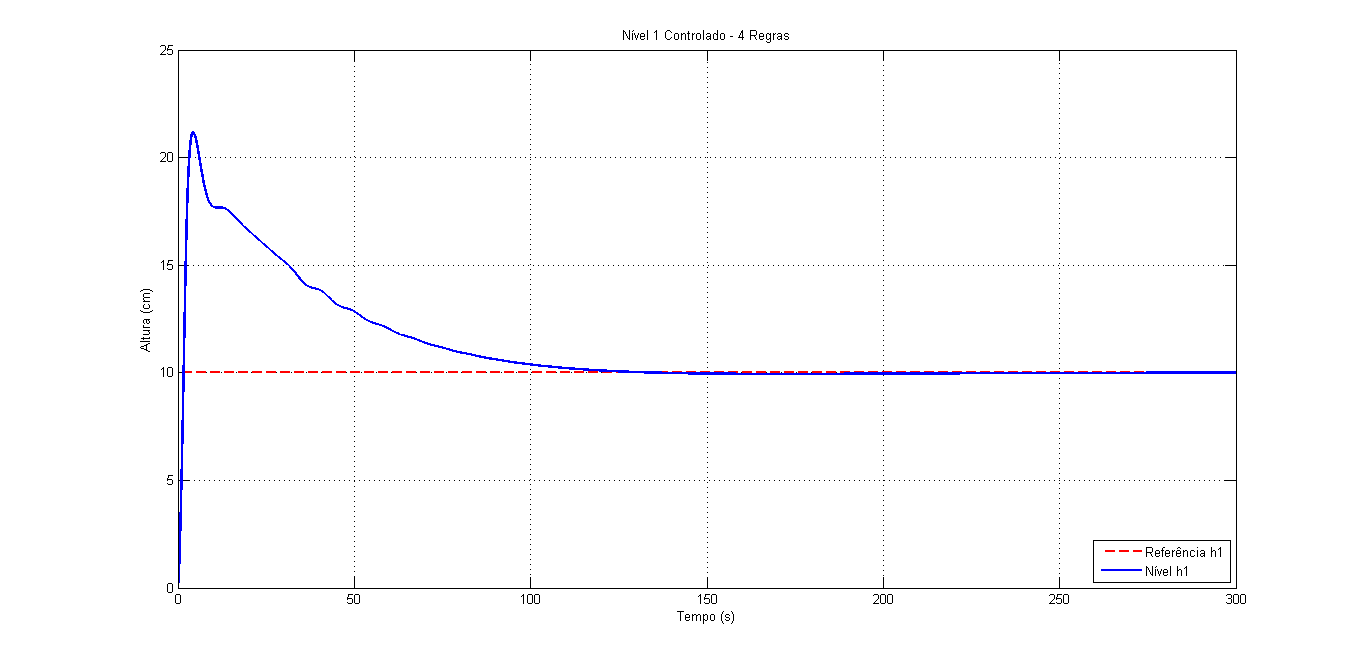
\includegraphics[width=\textwidth]{img/nm_ctrl_h2ts2_free.png}
	\caption{Nível H2 Controlado }
	\label{figH2CtrlTS2_free_nm}
\end{figure}

No entanto, é importante notar que o controle desenvolvido até aqui não leva em consideração os limites(5 V) dos atuadores (bomba). Incluindo-a ao modelo, tem-se:

Para os sistemas das \jhhref{imgTS5}{imagens} e \ref{imgTS15} são sintonizados de forma similar 15 e 225 ganhos e aplicados ao sistema. As imagens a seguir ilustram os resultados obtidos:
\begin{figure}[H]
	\centering
	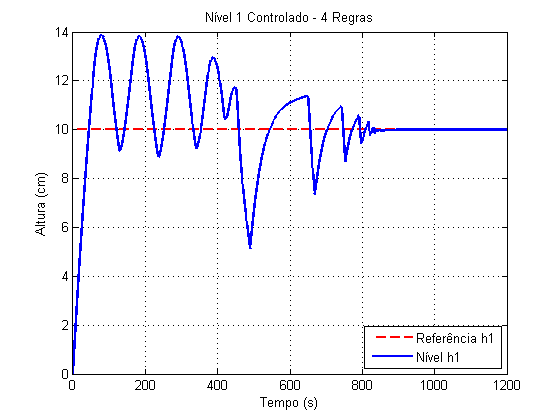
\includegraphics[width=\textwidth]{img/nm_ctrl_h1ts2_ulim.png}
	\caption{\small Nível H1 Controlado - Com saturação do Controlador }
	\label{figH1TSCtrl2_ulim_nm}
\end{figure}

\begin{figure}[H]
	\centering
	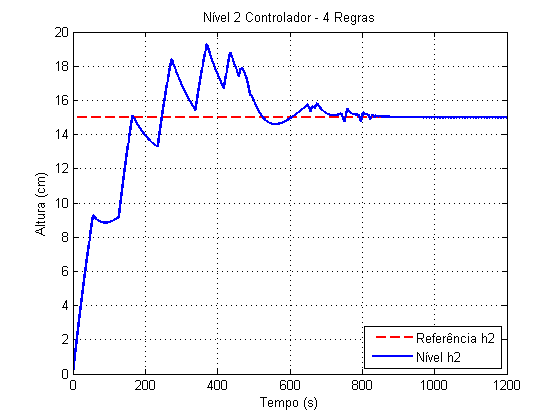
\includegraphics[width=\textwidth]{img/nm_ctrl_h2ts2_ulim.png}
	\caption{Nível H2 Controlado - Com saturação do Controlador }
	\label{figH2CtrlTS2_ulim_nm}
\end{figure}

Para aliviar a ultrapassagem, dada pelo efeito \textit{windup}, utiliza-se a saturação simples dos integradores nos momentos em que as variáveis manipuladas alcançam seus limites de atuação. Os gráficos a seguir ilustram:
\begin{figure}[H]
	\centering
	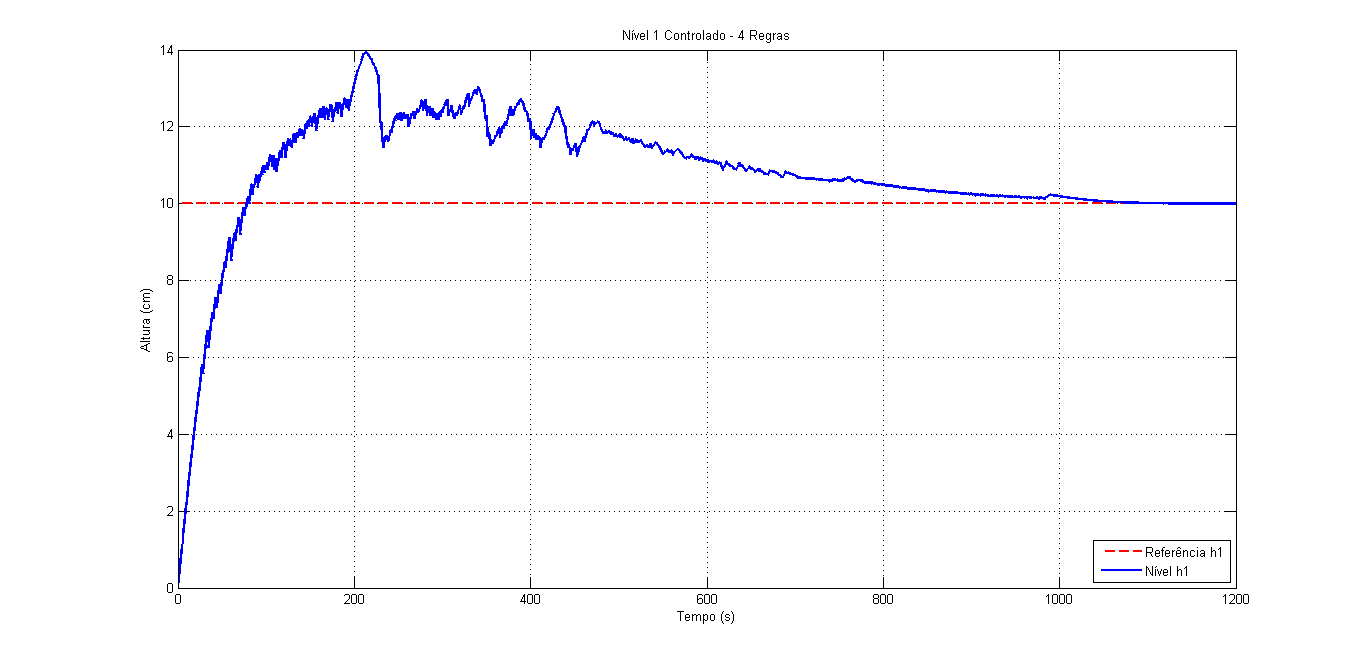
\includegraphics[width=\textwidth]{img/nm_ctrl_h1ts2.png}
	\caption{\small Nível H1 Controlado - Com \textit{Anti-Windup}}
	\label{figH1TSCtrl2_nm}
\end{figure}

\begin{figure}[H]
	\centering
	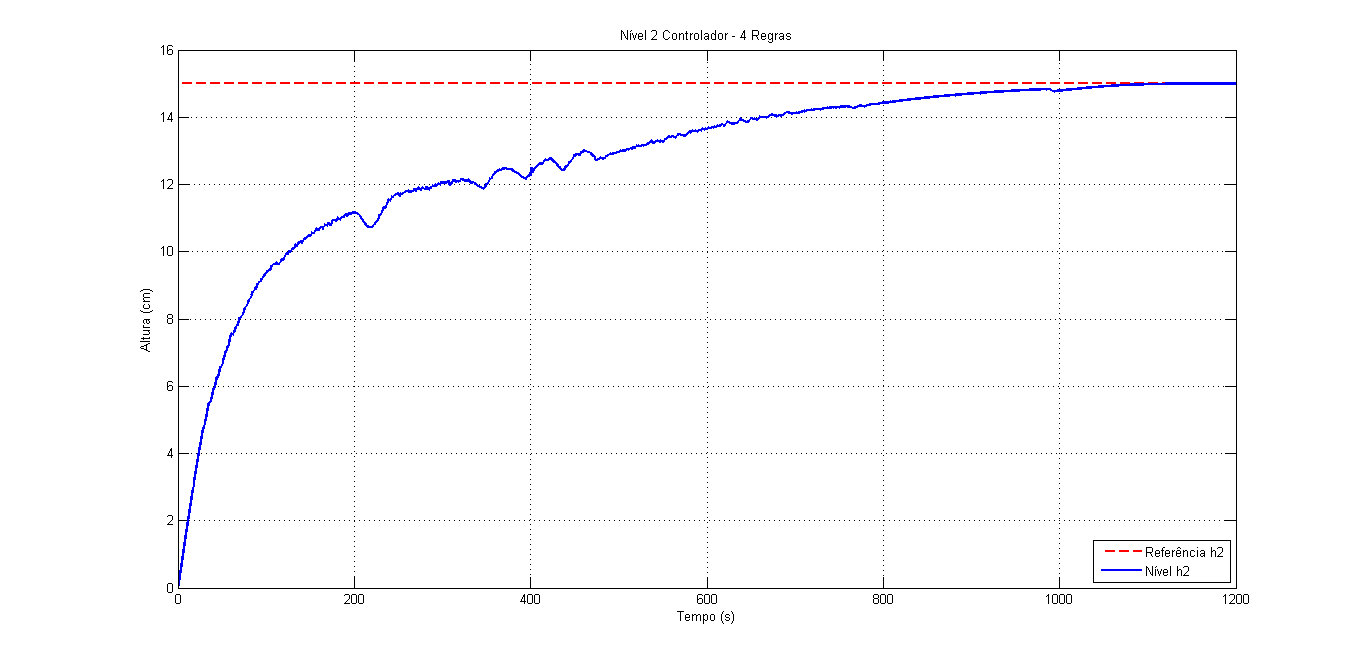
\includegraphics[width=\textwidth]{img/nm_ctrl_h2ts2.png}
	\caption{Nível H2 Controlado - Com \textit{Anti-Windup}}
	\label{figH2CtrlTS2_nm}
\end{figure}

\section{Implementação na Bancada} \label{secResImp}
Seguindo os procedimentos descritos no \jhhref{capImp}{Capítulo}, os ganhos obtidos na \jhhref{tabGanhosReais}{Tabela} são implementados e um degrau de referência para as alturas $h1=15$ e $h2=15$, observa-se:
\begin{figure}[H]
	\centering
	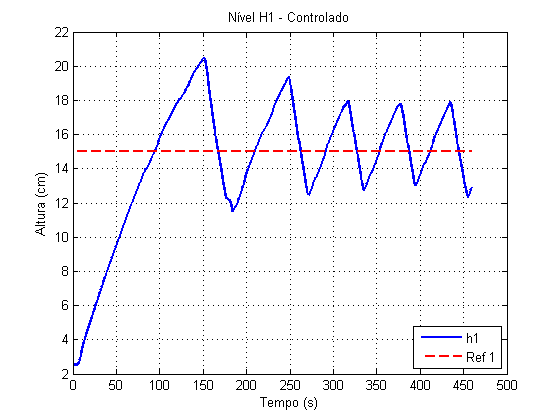
\includegraphics[height=0.35\paperheight,keepaspectratio]{img/ctrl_realh1.png}
	\caption{\small Nível H1 Controlado - Real}
	\label{imgH1Real}
\end{figure}

\begin{figure}[H]
	\centering
	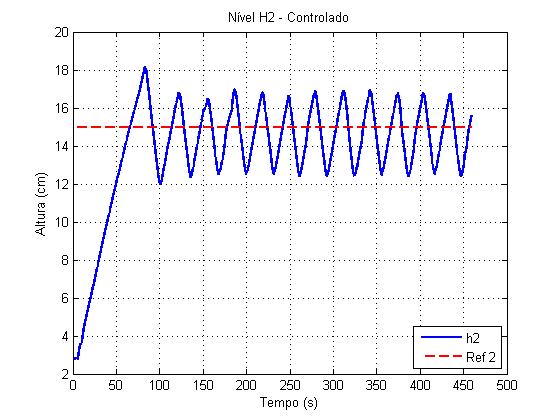
\includegraphics[height=0.35\paperheight,keepaspectratio]{img/ctrl_realh2.png}
	\caption{Nível H2 Controlado - Real}
	\label{imgH2Real}
\end{figure}

Nota-se que o comportamento geral do sistema tende a se estabilizar em torno da referência desejada. A forma oscilatória da resposta, não prevista no modelo, ocorre principalmente porque apesar do sinal de controle enviado, as bombas possuem uma zona de atuação que começa a funcionar apenas para sinais superiores à 30\%. Isso faz com que o erro continue aumentando até que se obtenha entradas superiores à este valor, o que gera a resposta observada.

\selectlanguage{brazil}%

